
\section{MIC implementation}
One of the most important factors to take into consideration when implementing photovoltaic (PV) modules is to obtain the maximum energy possible out of the available hardware, if this is not done, energy that should have been obtained will instead be lost. Since energy (E) is equal to power (P) over time (t), power must be maximized when the energy is being extracted. To achieve such goal a maximum power point tracker needs to be implemented, this is an electrical system that is always on the search of the location of the point where power extraction can be peaked. 
\begin{figure}[htbp]
	\begin{center}
		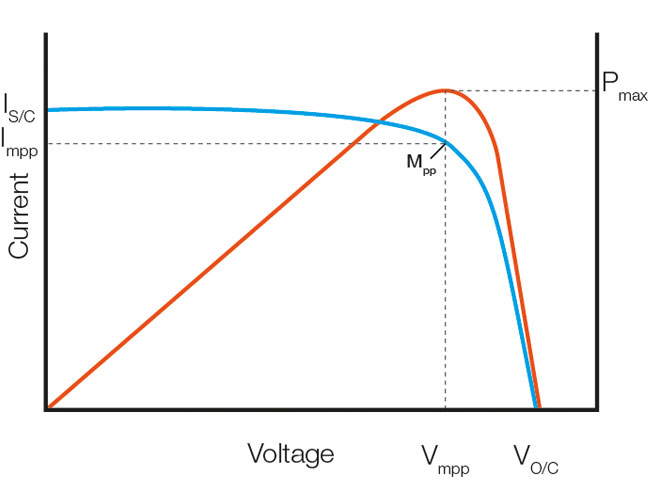
\includegraphics[width=0.6\linewidth]{../Pictures/mpp_graph.jpg}
		\caption{Maximum Power Point of generic solar panel.}
		\label{fig:mpp}
	\end{center}
\end{figure}

%[http://www.seaward-groupusa.com/userfiles/curve-tracing.php]%

MPPTs mostly consist on a power circuit that regulates either voltage drop or current flow across the PV terminals. There are many kinds of circuits that can be used to follow the maximum power point (MPP) of the PV, this topic will be further introduced in section blabla. 
However, solar plants and domestic used installations are composed of many modules, these modules are then connected to each other in series, parallel or in antiparallel configurations. To simplify the system, one MPPT is commonly used for many modules, this approach may lead to imperfections in the efficiency rates since the lower power generation of one module will then produce imperfections in the tracking system. 
This project focuses on the implementation of module integrated dc-dc converters (MICs). Using MICs for each module results in higher overall efficiencies, with this technology, events like partial shading, uneven dirt or wear distribution or imperfections produced in the assembly line are reduced and do not affect the rest of the modules in a line. Also, a more detailed control of the plant is achieved since separate data from each individual panel is obtained.
Different implementation options for MIC devices are possible but the most important objective of these devices is to individually control each module, resulting on an overall better efficiency rate, as well as a more robust system against any kind of inclemency. Each PV module will then be connected directly to each MIC, with this setup the output voltage and current are regulated by the device that extracts the energy, either an inverter, a battery or a load, allowing the system to work at different voltage and current levels whilst maintaining the MPP at all time.



